\documentclass[a4paper, 11pt, UTF8]{ctexart}
\usepackage{graphicx}
\usepackage{enumerate}
\usepackage{amssymb}
\usepackage{amsmath}
\usepackage{geometry}
\usepackage{caption}
\usepackage{subfigure}
\usepackage{float}
\usepackage{listings}
\usepackage{xcolor}
\usepackage{fontspec}
\usepackage{ulem}
\usepackage{hyperref}

\hypersetup{hidelinks}

\lstset{
    numbers=left,
    numberstyle= \tiny, 
    keywordstyle= \color{ blue!70},
    commentstyle= \color{red!50!green!50!blue!50}, 
    frame=shadowbox,
    rulesepcolor= \color{ red!20!green!20!blue!20} ,
    escapeinside=``,
    xleftmargin=2em, aboveskip=1em,
    framexleftmargin=2em,
    breaklines=true
}

\title{计算机程序设计基础大作业\\实验报告}

\author{机械108 \qquad 张益铭 \qquad 2021010552}

\date{2022年5月24日}

\geometry{left=3cm, right=3cm, top=4cm, bottom=4cm}

\begin{document}

\maketitle

\tableofcontents

\rightline{p.s. 点击目录进行跳转 :)}

\newpage

\section{实现功能及整体框架}

\subsection{实现功能}

本次大作业选题为大数计算器,实现了\textbf{基本功能}和\textbf{进阶功能},这两个功能在一个程序中实现。

其中,基本功能能够对用户输入的加、减、乘以及求余数($+, -, *, \% $)表达式进行计算,
取值范围为int范围内的整形数字,最终返回一个在long long范围内的结果。

进阶功能是实现两个较大数字的乘法运算,理论上可以计算数字位数在int范围内的两数相乘,实际可能需要进行输入输出重定向。

\subsection{整体框架}

此次大作业代码模块化程度较高,主要分为输入处理部分、判断输入表达式合法性、基本功能的实现以及进阶功能的实现。
总共有一个*.h头文件和五个*.cpp源文件,总代码量为400行左右,使用GBK格式编码,注释、命名、分块较为合理。

\subsubsection{函数声明}

本次大作业使用的函数均在my\_function.h中进行声明,其中包含相关库的调用以及部分变量的声明,具体内容如下图所示。

\begin{figure}[H]
    \centering
    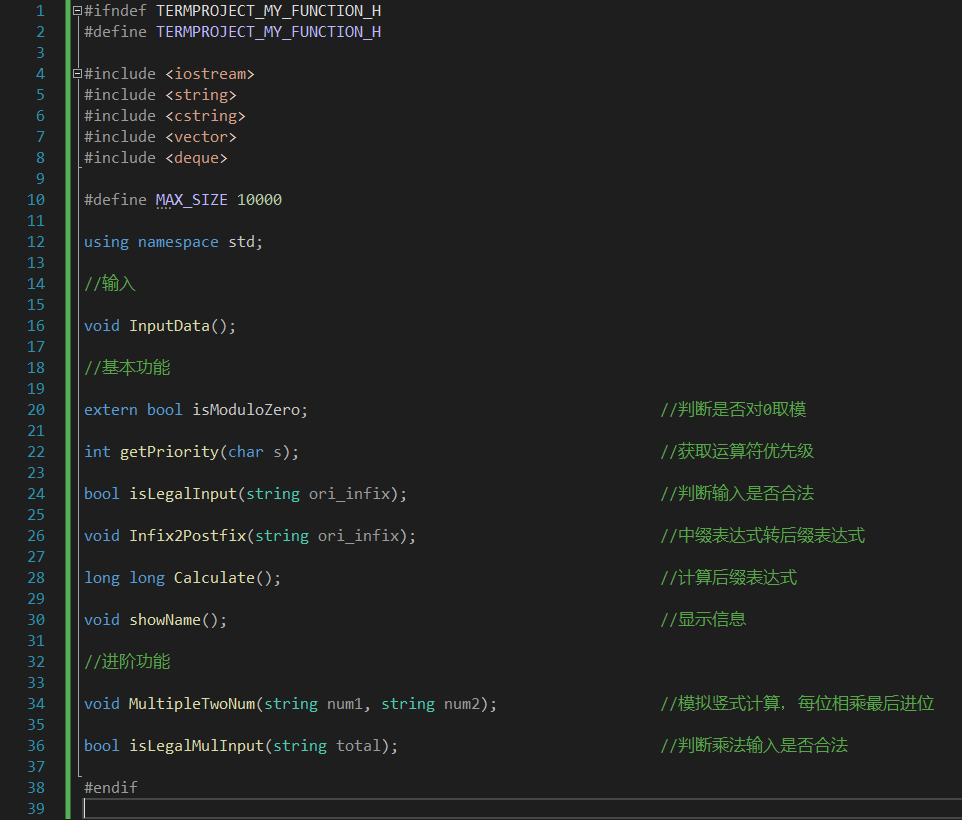
\includegraphics[width=0.7\textwidth]{my_function}
    \caption{my\_function.h}
\end{figure}

\subsubsection{主函数}

主函数main.cpp内容较简单,内含注释表明个人信息。main函数调用showName()和Input()函数,具体功能见后续介绍。

\begin{lstlisting}[language=C++, basicstyle=\ttfamily]
 //
 //Term Project of Programming Fundamentals.
 //Created by 张益铭 2021010552 on 4/13/2022.
 //Copyright (C) 张益铭 2022. All Rights Reserved.
 //Encoding with GBK.
 //

 #include "my_function.h"

 int main() {
    showName();
    
    Input();
    
    system("pause");
    return 0;
 }    
\end{lstlisting}

\subsubsection{输入处理}

输入处理工作主要由Input.cpp实现。

Input.cpp里的Input()函数(第3行)会对输入数据进行处理。用户需要先选择功能类型,1代表Basic Function(基本功能),2代表Advanced Function(进阶功能)。
随后程序会提示用户输入相应表达式,若表达式合法,将会调用相应的计算功能函数,否则会提示“Invalid function type!”。

\subsubsection{判断输入合法性}

判断输入合法性主要由Judgement.cpp实现。

Judgement.cpp中包含两个bool类型函数:isLegalInput()函数(第5行)和isLegalMulInput()函数(第91行),分别判断基本功能和进阶功能的表达式合法性。
若表达式合法,将会返回true并进行计算,否则会给出具体出错提示,并返回false。

\subsubsection{基本功能}

基本功能主要由BasicFunc.cpp实现。

包括getPriority()(第11行),Infix2Postfix()(第28行),Calculate()(第84行)、showName()(第133行)等函数,分别实现获取运算符优先级、
将输入的中缀表达式转化为后缀表达式、计算后缀表达式以及显示本人信息的功能。

\subsubsection{进阶功能}

进阶功能主要由AdvancedFunc.cpp实现。

包含MultipleTwoNum()(第3行)函数,负责计算两个大数相乘,主要通过模拟竖式计算实现。

\section{设计及实现思路}

\subsection{显示个人信息}

运行该程序后,先调用showName()函数,显示个人信息,该函数在BasicFunc.cpp中定义,较简单故不再赘述。

\begin{figure}[H]
    \centering
    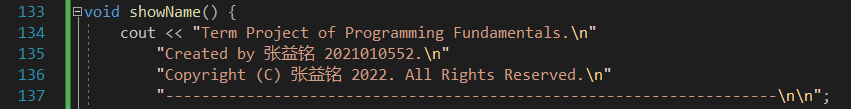
\includegraphics[width=\textwidth]{showname}
    \caption{showName()}
\end{figure}

其次调用Input(),处理输入。

\subsection{处理输入}

功能选择的合法的输入为1和2,对应基本和进阶功能。为区分不合法输入,本人使用string类变量whichFunc来记录用户选择,考虑到可能的错误如下:

\begin{enumerate}[a)]
    \item 输入字符串长度不为1
    \item 字符串长度为1,但不是1或2
\end{enumerate}

对于a,直接输出"Invalid function type!",程序结束;对于b,使用switch来扫描whichFunc[0],default项为输出"Invalid function type!"。

对于上述switch函数,case '1'为基本功能。
若表达式合法,即通过isLegalInput()的检验,再使用Infix2Postfix()将输入的中缀表达式转化为后缀表达式进行计算,
若运算中没有出现对0取余的情况,则输出结果res。

\begin{lstlisting}[language=C++, basicstyle=\ttfamily]
 case '1': {
    string ori_infix;

    cout << "Basic Func Mode.\n"
        "Please enter the expression:\n";
    getline(cin, ori_infix);

    if (isLegalInput(ori_infix)) {
        Infix2Postfix(ori_infix);
        long long res = Calculate();
        if (!isModuloZero) {
            cout << "The result is:\n" << res << endl;
        }
    }
    break;
 }   
\end{lstlisting}

case '2'项对应进阶功能。
考虑到long long也装不下待计算数字,故定义string类变量num1和num2对应第一和第二个乘数。表达式通过isLegalMulInput()的检验后,会被分割为两个乘数。

遇到空格或*前使用.push\_back()存入第一个数,遇到空格和*后开始存入第二个数。关于是否到第二个数,我定义了bool类型变量isNum2来判断,部分代码如下。

\begin{lstlisting}[language=C++, basicstyle=\ttfamily]
 bool isNum2 = false;

 for (char i : total) {
	if (i == '*' || i == ' ') {
		isNum2 = true;
	}
	if (!isNum2) {
		num1.push_back(i);
	}
	else if (i != '*' && i != ' ') {
		num2.push_back(i);
	}
 }
\end{lstlisting}

\subsection{基本功能}

关于表达式合法性检测,我会在后文解释,现在我们假定输入均为合法输入。

考虑到中缀表达式并不利于计算机处理,并且受到PA08中3039后缀表达式作业的启发,我先将中缀表达式转化为后缀,再模仿栈的运行方式进行计算。

\subsubsection{获取运算符优先级}

由getPriority()完成。
由于遇到'('时入栈,直到遇到')'时将栈内运算符全部弹出,故定义'('优先级为1,'+'、'-'为2,'*'、'\%'为3,')'最高,为4,
并默认数字优先级为0。

\subsubsection{中缀转后缀}

由Infix2Postfix()完成。预处理:为处理负数,我将其改为0 - 正数,即在符号前加入一个0,这样就能进行负数的输入,并且为了方便转化以及避免不必要的麻烦,
我在转化前遍历中缀表达式清除了其中的空格。

转化的主要思路是遍历中缀,遇到数字则存入后缀表达式,遇到运算符则存入vector容器op中,模拟栈的运行。
若遇到的运算符优先级小于上一个,则上一个运算符出栈,存入后缀,该运算符入栈,遍历完成后将栈内元素清空。
伪代码示意图如下:

\begin{figure}[H]
    \centering
    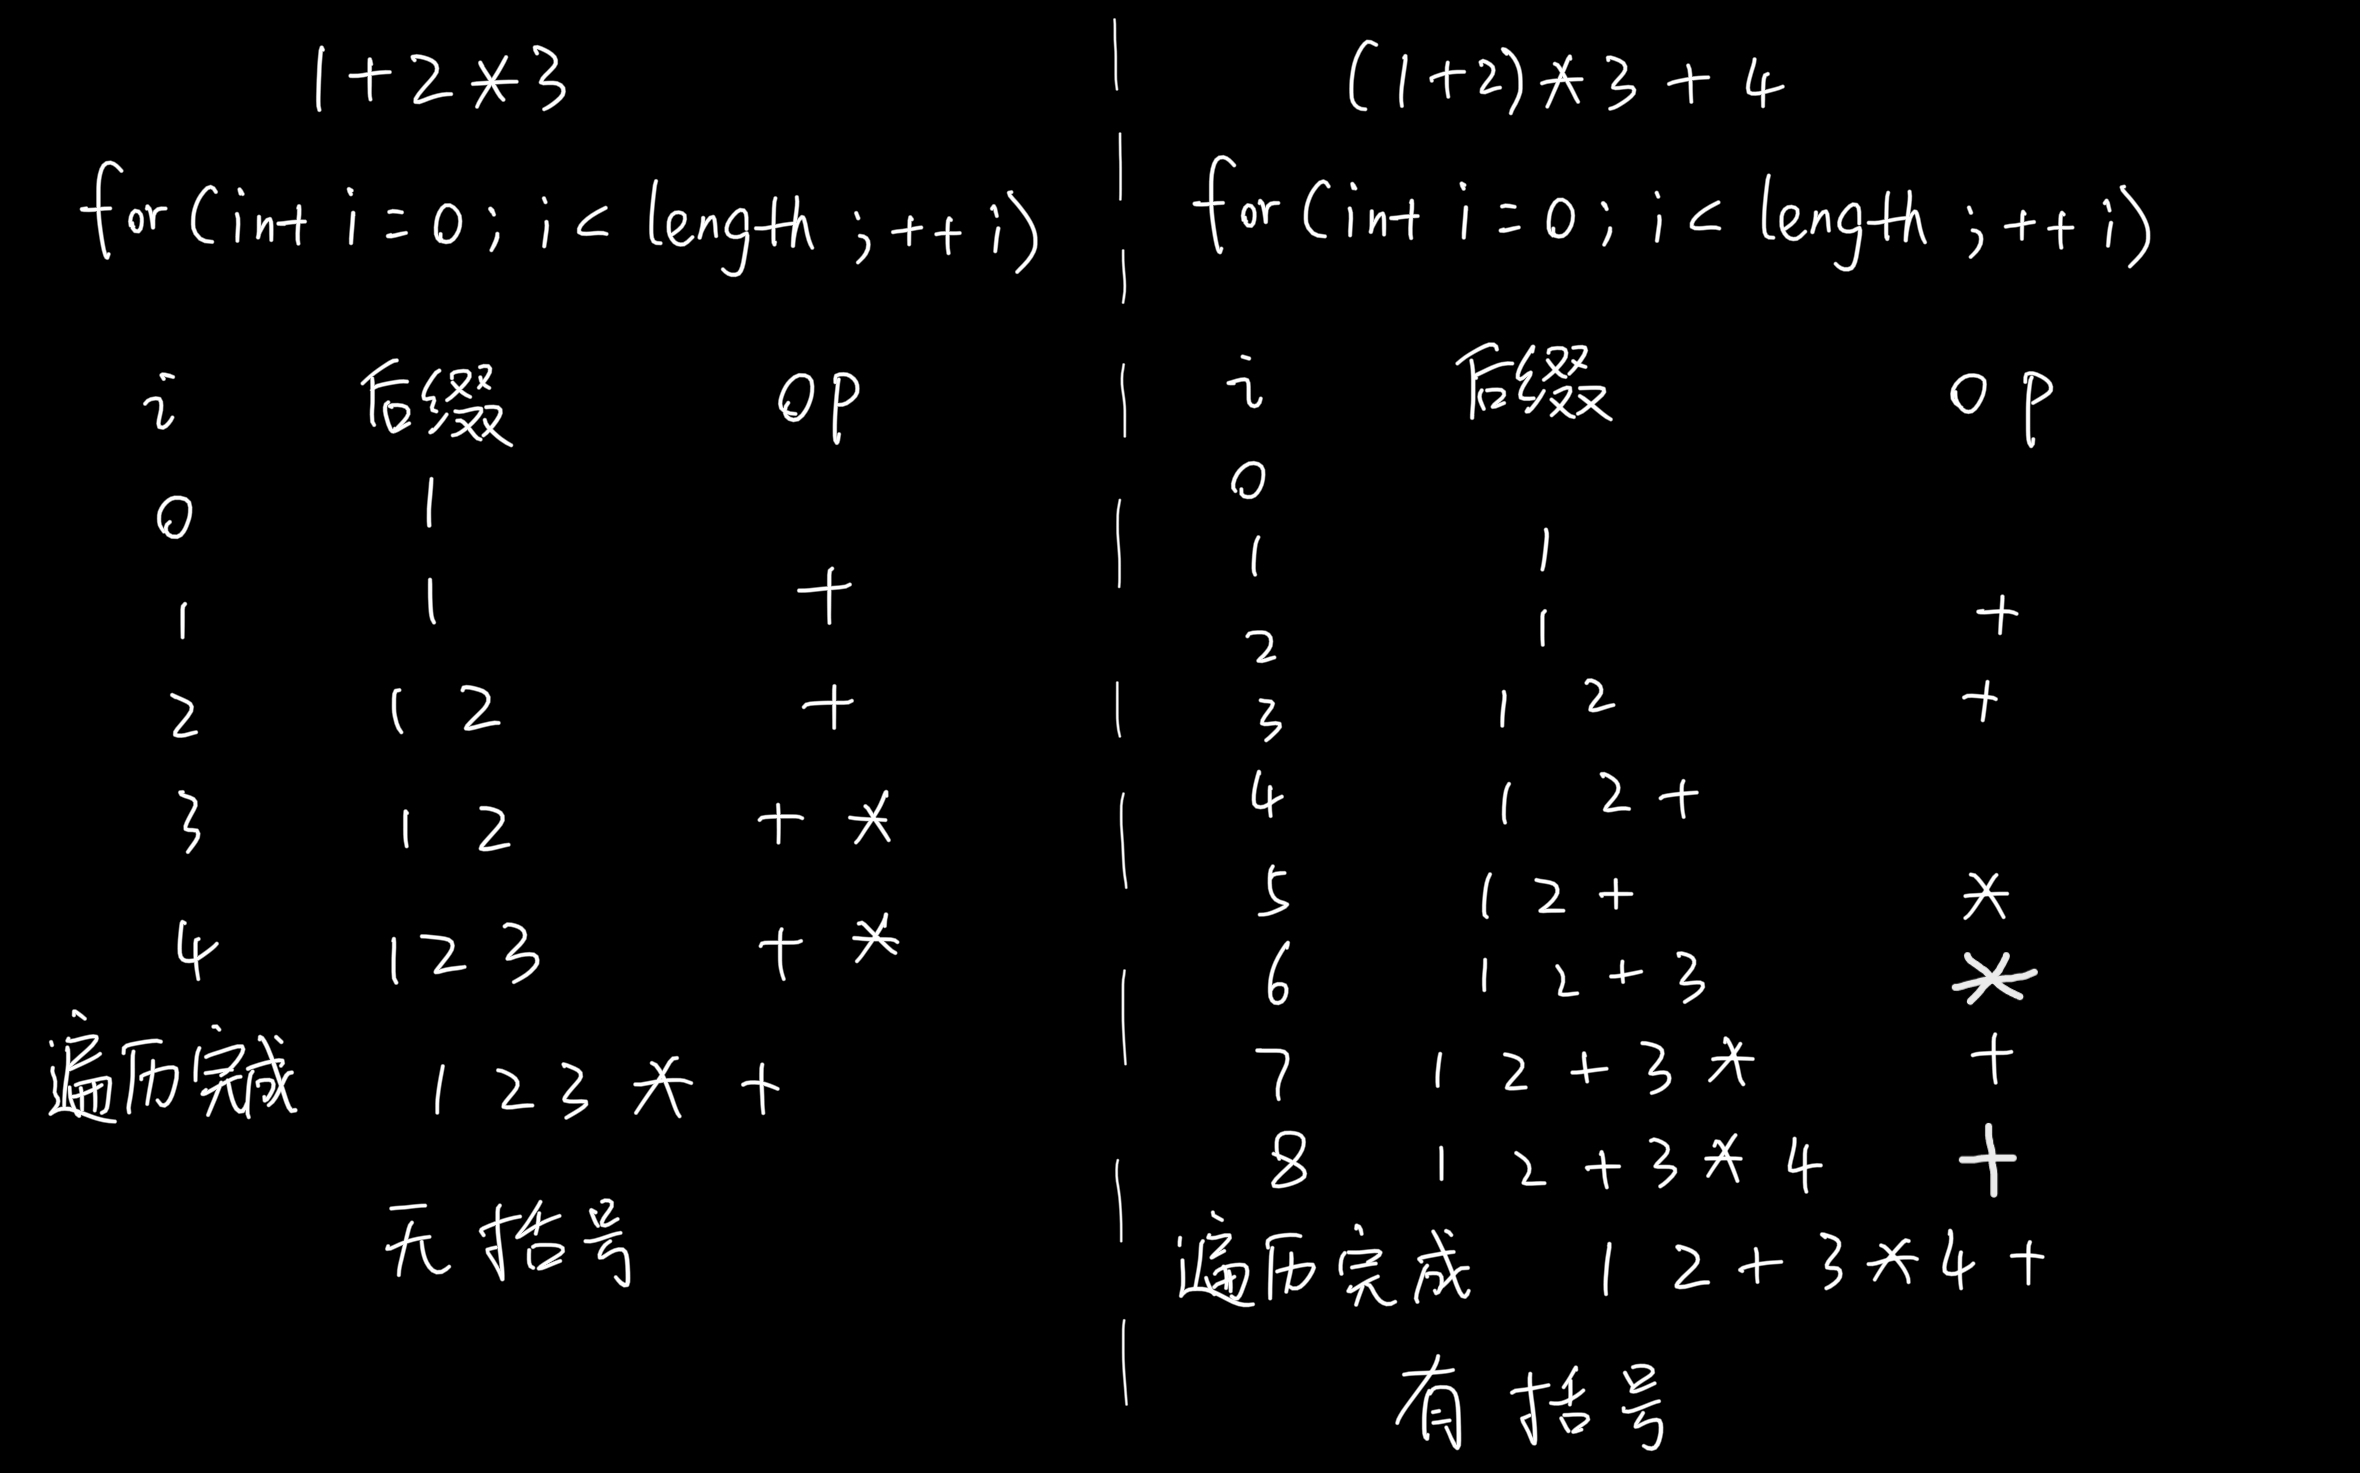
\includegraphics[width=0.7\textwidth]{infix2postfix.jpg}
    \caption{中缀转后缀示意图}
\end{figure}

\textit{*转化的后缀表达式存储在BasicFunc.cpp中的char型全局数组postfix中。}

\subsubsection{计算后缀表达式}

由Calculate()完成。
由于计算的结果在long long范围,int数组并不能满足,故我定义了一个结构体Stack,用来作为“long long数组”存储数据,
并使用vector容器创建stack变量 \verb|vector<Stack> stack(MAX_SIZE);|。

\begin{lstlisting}[language=C++, basicstyle=\ttfamily]
 struct Stack { 
	long long s;
 };
\end{lstlisting}

思路是遇到数则压入栈中,遇到运算符则计算栈顶的前两个数字,栈顶元素出栈。
为防止对0取余,我定义了一个全局bool变量isModuloZero,检测到\%时判断栈顶元素是否为0,如果为0则将isModuloZero赋值为true,并输出“Modulo 0!”,
反之正常计算。

考虑到用户可能只输入一个数字,按照上述方法则不能输出该数字,所以在遍历完成时需检测num是否为0,若不是则将num作为结果输出。

\begin{lstlisting}[language=C++, basicstyle=\ttfamily]
 int j = 0;  //模拟控制入栈出栈
 for (int i = 0; i < strlen(postfix); ++i) {
    if (postfix[i] >= '0' && postfix[i] <= '9') {
        num = num * 10 + postfix[i] - '0';
    }
    else {
        if (num != 0 || (i >= 1 && postfix[i - 1] == '0')) {
            //防止负号前补充的0被忽略
            stack[j++].s = num;
            num = 0;
        }
        if (j >= 2) {
            ......  //进行运算
        }
    }
 }
 if (num != 0) {
    stack[j].s = num;
 }
\end{lstlisting}

\subsection{进阶功能}

进阶功能的实现较为简单,可以通过模拟竖式计算来完成。为了便于队首及队尾元素的增删,我使用了deque容器。

\subsubsection{各个数位交叉相乘}

我先将每位元素相乘到对应数位,最后统一处理进位。

\begin{lstlisting}[language=C++, basicstyle=\ttfamily]
 for (int i = 0; i < num1.length(); ++i) {
    for (int j = 0; j < num2.length(); ++j) {
        result[i + j] += (num1[i] - '0') * (num2[j] - '0');
    }
 }
\end{lstlisting}

\subsubsection{处理进位}

关于进位问题,主要思路为遍历未处理进位的result,定义一个int型carry变量,存储上一位进上来的数,随后carry更新为result[i]除以10,即在十位之上的数字,
最后将每一位数先加上carry再对10取余,至此就完成了进位问题。

但是这种方法有一种不足之处,即无法对最高位进行进位,这也是我使用deque容器而不是vector的原因,因为vector只能处理末尾,不能对首位进行增删操作。

\subsubsection{修补最高位}

对最高位进行进位也较为简单,大致思路为使用while判断carry是否为0,若是则保留carry的个位为最高位,将十位以上的数继续向上进位,直到carry为0为止。

\begin{lstlisting}[language=C++, basicstyle=\ttfamily]
while (carry != 0) {
	int temp = carry % 10;
	result.push_front(temp);
	carry /= 10;
 }
\end{lstlisting}

同时为了防止最高位出现0,即会出现010*2=020的情况,所以当结果不为0时会使用while删除最高位的0,避免输出出错(此处省略代码)。

p.s. 最开始提到“理论上可以计算数字位数在int范围内的两数相乘”,其中的int范围限制可以通过改变循环变量i的类型,例如改为long long类型来实现更多数位的计算。

\subsection{程序鲁棒性}

\sout{众所周知,写代码5分钟,debug两小时},为了避免各种可能的异常输入导致程序崩溃,我想到了如下了可能出现的异常。

\begin{table}[H]
    \centering
    \begin{tabular}{|ccc|}
        \hline
        \multicolumn{3}{|c|}{\textbf{可能的输入异常}}                                           \\ \hline
        \multicolumn{1}{|c|}{}  & \multicolumn{1}{c|}{\textbf{基本功能}}    & \textbf{进阶功能} \\ \hline
        \multicolumn{1}{|c|}{1} & \multicolumn{1}{c|}{是否输入}             & 是否输入          \\ \hline
        \multicolumn{1}{|c|}{2} & \multicolumn{1}{c|}{第一位不是数字}       & 乘数个数          \\ \hline
        \multicolumn{1}{|c|}{3} & \multicolumn{1}{c|}{英文/中文符号}        & 乘号个数          \\ \hline
        \multicolumn{1}{|c|}{4} & \multicolumn{1}{c|}{输入不是数字}         & 是否是乘号        \\ \hline
        \multicolumn{1}{|c|}{5} & \multicolumn{1}{c|}{缺少/多余/错误运算符} & \textbackslash{}  \\ \hline
        \multicolumn{1}{|c|}{6} & \multicolumn{1}{c|}{多/少括号}            & \textbackslash{}  \\ \hline
        \multicolumn{1}{|c|}{7} & \multicolumn{1}{c|}{对0取余}              & \textbackslash{}  \\ \hline
    \end{tabular}
\end{table}

注:为了避免不必要的麻烦,在两种检测功能最开始都会遍历输入,删除其中的空格,之后遇到任何一种错误都会给出提示并返回false,
只有通过全部检验才回返回true,进行后续计算。

\subsubsection{基本功能输入异常}

基本功能需考虑的异常相对较多,我将按照上述顺序依次介绍相关处理思路。

\begin{enumerate}
    \item 对于是否输入,只需检测长度是否为0,若为0,立即显示“Please enter the expression!”,程序结束。
    \item 一般情况下,表达式中第一位都是数字或者括号,只有输入的第一数为负数时才会出现运算符,因此若第一位是“+,*,\%”中的一种,
          都会提示“Operator missing operand!”。但是只输入一个符号也是不行的,因此如果表达式长度为1并且第一位是符号也会报错。
    \item 由于计算表达式中含有括号,部分用户可能输入中文输入法下的括号,造成输入异常。经测试知,‘(’和‘(’对应的ASCII码并不相同,
          中文每个汉字由两个及以上字节组成,具体表现为其ASCII码小于0,因此在遍历过程中遇到某位的ASCII码小于0
          就会提示“Please enter expressions in English!”
    \item 当输入不是数字时,则必须是合法运算符中的一种,所以在遍历中使用了switch函数判断输入不是数字的情况。
          \begin{lstlisting}[language=C++, basicstyle=\ttfamily]
if (ori_infix[i] < '0' || ori_infix[i] > '9') {
    switch (ori_infix[i]) {
		case '(':
		case ')':
		case '+':
		case '-':
		case '*':
		case '%':
			break;
		default:
			cout << "Invalid operator!\n";
			return false;
	}
}
          \end{lstlisting}
    \item 对于输入运算符错误,可能的情况有:连续多个加减乘取余符号、除了负数之外的左括号连接运算符(不包括连续多个左括号)、
          运算符连接右括号(不包括连续多个右括号)等问题,发现一种都会输出“Operator missing operand!”
    \item 多/少括号的判断则比较简单,只需统计左右两种括号的个数,二者不相等就会输出“Parenthesis DO NOT match!”
    \item 关于判断是否对0取余,已经在Calculate()中进行了介绍,不再赘述。
\end{enumerate}

\subsubsection{进阶功能输入异常}

进阶功能输入异常相对较少,主要如下。

\begin{enumerate}
    \item 对于是否是输入,处理方法同基本功能。
    \item 若第一位是'*',说明未输入第一个乘数,会提示“Please enter the first multiplier!”,如果表达式最后一位是'*',
          说明未输入第二个乘数,提示“Please enter the second multiplier!”
    \item 统计乘号个数,如果不唯一则提示“You can ONLY multiply two numbers!”
    \item 由于进阶功能的输入只有数字和乘号,所以对于数字之外的输入,如果是乘号,则乘号个数+1,
          否则输出“You can ONLY enter multiplication signs or numbers!”
\end{enumerate}

\section{使用说明及实现效果}

注:相关输入要求见readme.txt

\subsection{开始}

首先,程序会提示用户选择功能类型(1代表Basic Function,2代表Advanced Function).

\begin{figure}[H]
    \centering
    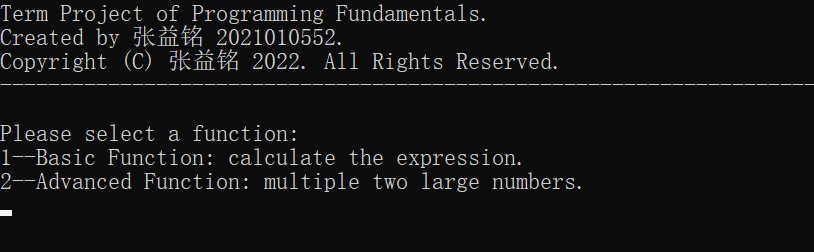
\includegraphics[width=0.96\textwidth]{begin.png}
    \caption{选择功能}
\end{figure}

选择完毕后程序会显示当前的功能,并提示输入表达式。

\begin{figure}[H]
    \centering
    \begin{minipage}[t]{0.48\textwidth}
        \centering
        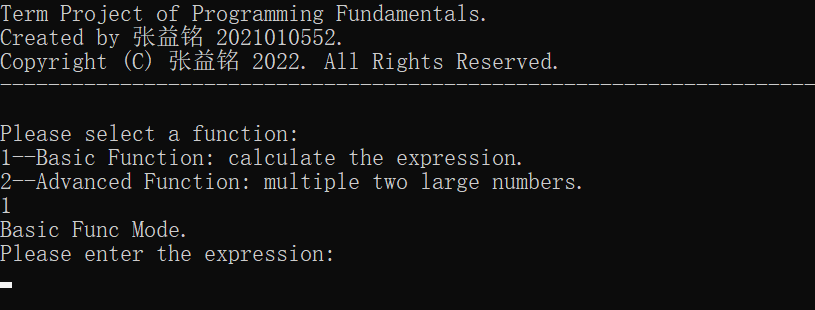
\includegraphics[width=7cm]{func1.png}
    \end{minipage}
    \begin{minipage}[t]{0.48\textwidth}
        \centering
        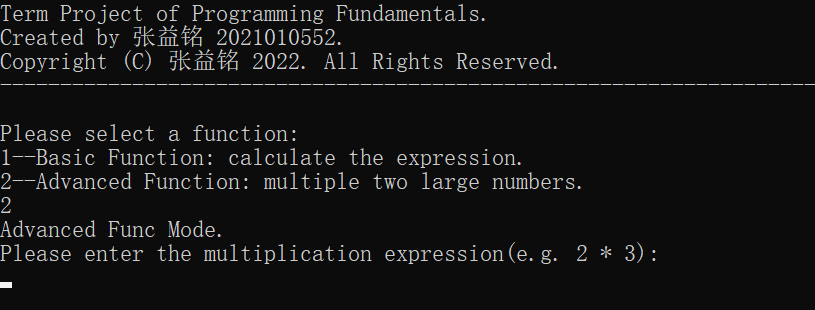
\includegraphics[width=7cm]{func2.png}
    \end{minipage}
    \caption{两种功能页面}
\end{figure}

\subsection{功能1:基本功能}

用户在基本功能里可以输入加、减、乘、取余表达式,能够进行括号运算,数字内部不可以有空格,两个数之间可以有任意数量的空格,
输入完成按下enter后,会显示“The result is:”并输出结果,部分输入结果如图。

\begin{figure}[H]
    \centering
    \subfigure{
        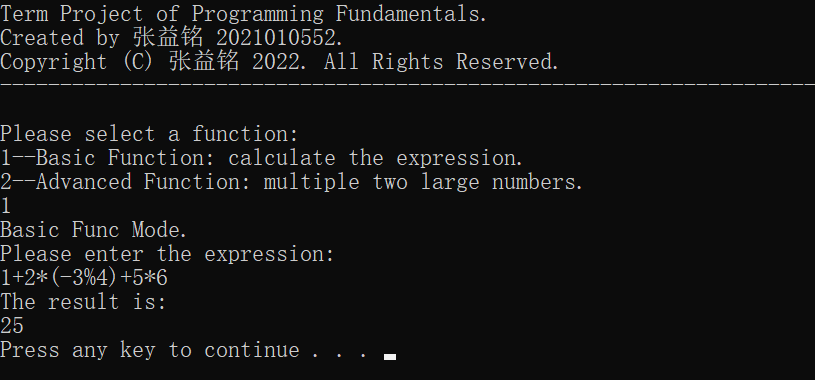
\includegraphics[width=0.65\textwidth]{res11.png}
    }
    \quad
    \subfigure{
        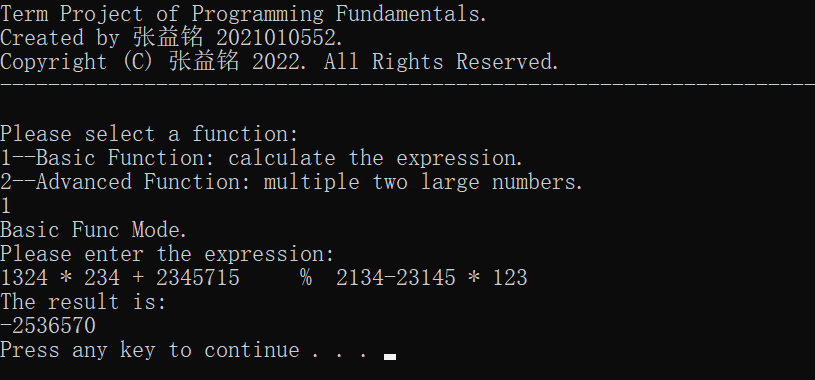
\includegraphics[width=0.65\textwidth]{res12.png}
    }
    \quad
    \subfigure{
        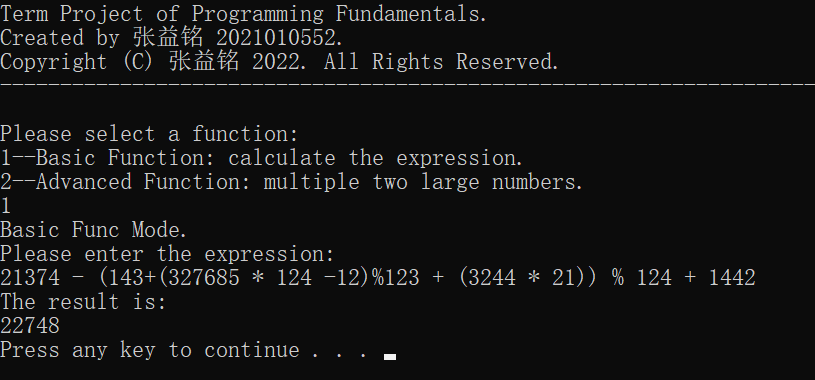
\includegraphics[width=0.65\textwidth]{res13.png}
    }
    \quad
    \subfigure{
        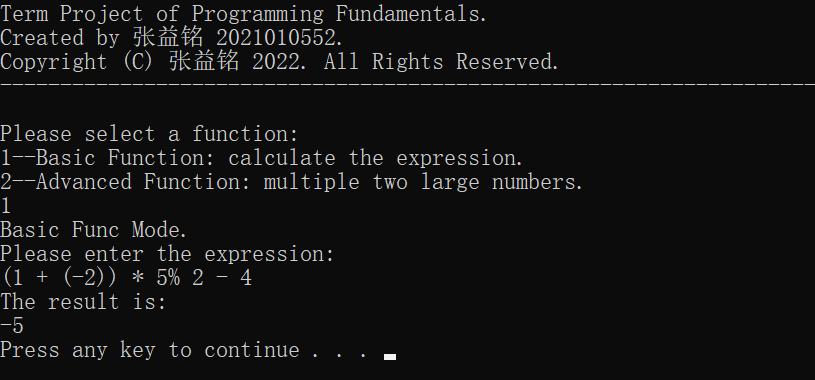
\includegraphics[width=0.65\textwidth]{res14.png}
    }
    \caption{部分输入案例}
\end{figure}

\subsection{功能2:进阶功能}

进阶功能用户可计算两个大数的乘法,其中数字的位数应该在int范围内(远远满足作业100000位的要求),且两个数应均为非负数,
输入完成按下enter后,会显示“The result is:”并输出结果,部分输入结果如图。

\begin{figure}[H]
    \centering
    \subfigure{
        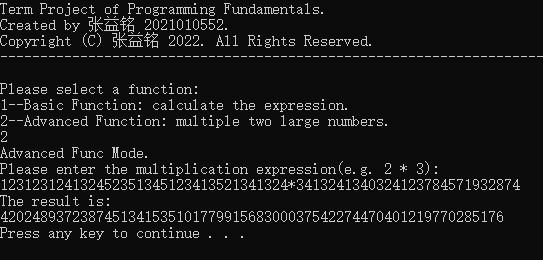
\includegraphics[width=0.7\textwidth]{res21.png}
    }
    \quad
    \subfigure{
        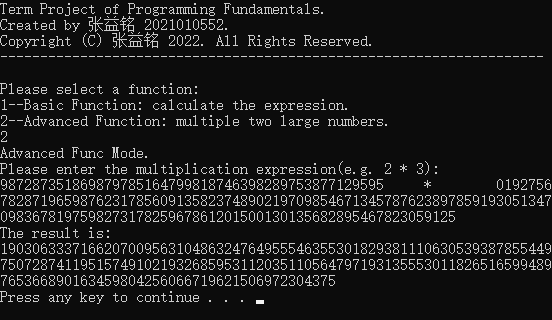
\includegraphics[width=0.7\textwidth]{res22.png}
    }
    \quad
    \subfigure{
        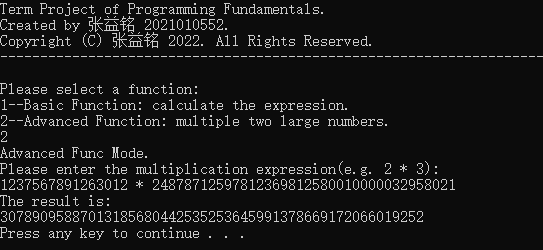
\includegraphics[width=0.7\textwidth]{res23.png}
    }
    \caption{部分输入案例}
\end{figure}

\end{document}
